\chapter{Polimer: Sintesis, Struktur, dan Sifat}\label{ch:b2:polymer-synthesis}

Stoking nilon mulai dijual pada tahun 1939. Stoking itu lahir dari sebuah
laboratorium yang beberapa tahun sebelumnya berusaha memahami bagaimana
molekul-molekul kecil bergabung menjadi molekul panjang, dan yang di
sepanjang jalan mendapat pelajaran yang mengejutkan setiap kimiawan pada
kali pertama: untuk \omterm{def:b2:polymer-synthesis:polymer}{polimer} yang dibuat dengan menyambungkan molekul-molekul
ujung ke ujung, rendemen 99~\% tidaklah cukup. Bab ini menjelaskan alasannya,
menguraikan kedua cara rantai tumbuh, dan menghubungkan struktur rantai
dengan sifat-sifat material.
% ledger: hist:nylon-production-1939

\begin{recall}
Jilid sekolah: \omterm{def:b2:polymer-synthesis:polymer}{polimer}, \omterm{def:b2:polymer-synthesis:polymer}{monomer} dan \omterm{def:b2:polymer-synthesis:polymer}{satuan ulang}, \omterm{def:b2:polymer-synthesis:polymer}{polimer} adisi dan \omterm{def:b2:polymer-synthesis:polymer}{polimer}
kondensasi, termoplastik dan termoset. Jilid Tahun 1: radikal dan homolisis,
karbokation dan karbanion, pendekatan keadaan tunak.
\Cref{ch:b2:acyl-substitution}: ester dan amida.
\Cref{ch:b2:catalytic-cycles}: insersi ke dalam ikatan logam--karbon.
\end{recall}

\section{Rantai dan massa molarnya}

\begin{definition}[Polimer]\label{def:b2:polymer-synthesis:polymer}
Yang disebut \emph{polimer}\index{polimer} adalah zat yang terdiri atas
makromolekul, yang masing-masing dibangun melalui penyambungan berulang
molekul-molekul kecil, yaitu \emph{monomer}\index{monomer}. Yang disebut
\emph{satuan ulang}\index{satuan ulang} adalah gugus atom terkecil yang
pengulangannya membentuk rantai; \emph{derajat
polimerisasi}\index{derajat polimerisasi} $X$ sebuah rantai adalah banyaknya
satuan turunan monomer yang dikandungnya.
\end{definition}

Sampel \omterm{def:b2:polymer-synthesis:polymer}{polimer} sintetis tidak pernah terdiri atas rantai-rantai yang
identik: sampel itu adalah campuran rantai dengan panjang yang berbeda-beda,
dan massa molarnya adalah rata-rata, yang bergantung pada cara rantai-rantai
itu dihitung.

\begin{definition}[Rata-rata massa molar]\label{def:b2:polymer-synthesis:averages}
Untuk sampel yang mengandung $N_i$ rantai bermassa molar $M_i$, \emph{massa
molar rata-rata jumlah}\index{massa molar rata-rata jumlah} dan \emph{massa
molar rata-rata massa}\index{massa molar rata-rata massa}
adalah
\begin{equation*}
\bar M_n = \frac{\sum_i N_i M_i}{\sum_i N_i}, \qquad
\bar M_w = \frac{\sum_i N_i M_i^2}{\sum_i N_i M_i} = \sum_i w_i M_i,
\end{equation*}
dengan $w_i$ fraksi massa rantai-rantai bermassa $M_i$. Yang disebut
\emph{dispersitas}\index{dispersitas}
$\text{\DH} = \bar M_w/\bar M_n$ sekurang-kurangnya bernilai 1, dan sama
dengan 1 hanya jika semua rantai mempunyai massa yang sama. Rata-rata $\bar X_n$
dan $\bar X_w$ \omterm{def:b2:polymer-synthesis:polymer}{derajat polimerisasi} didefinisikan dengan cara yang sama.
\end{definition}

Rata-rata jumlah memberi bobot satu kali pada setiap rantai; rata-rata
massa memberi bobot pada setiap rantai menurut massanya, sehingga
rantai-rantai panjang lebih diperhitungkan. Bahwa $\text{\DH} \ge 1$ adalah
ketaksamaan $\left(\sum N_i M_i\right)^2 \le
\sum N_i \sum N_i M_i^2$ (Cauchy--Schwarz), dengan kesamaan hanya untuk $M_i$ yang sama.

\begin{method}[Menghitung rata-rata]\label{met:b2:polymer-synthesis:averages}
\begin{enumerate}
  \item Ubahlah data menjadi jumlah $N_i$ (atau banyaknya rantai) dan massa
        $M_i$; dari fraksi massa,
        $N_i \propto w_i/M_i$.
  \item $\bar M_n = \sum N_i M_i / \sum N_i$; secara setara, $1/\bar M_n = \sum w_i/M_i$.
  \item $\bar M_w = \sum w_i M_i$.
  \item $\text{\DH} = \bar M_w/\bar M_n$; periksalah bahwa $\bar M_w \ge \bar M_n$.
\end{enumerate}
\end{method}

\section{Pertumbuhan bertahap dan pertumbuhan rantai}

\begin{definition}[Pertumbuhan bertahap dan pertumbuhan rantai]\label{def:b2:polymer-synthesis:step-chain}
Dalam \emph{polimerisasi pertumbuhan bertahap}\index{polimerisasi pertumbuhan bertahap},
setiap dua molekul yang membawa gugus fungsi yang saling melengkapi
(\omterm{def:b2:polymer-synthesis:polymer}{monomer}, oligomer, atau rantai panjang) dapat bereaksi, dan rantai-rantai
memanjang dengan saling bergabung: poliester, poliamida. Dalam
\emph{polimerisasi pertumbuhan
rantai}\index{polimerisasi pertumbuhan rantai}, sebuah pusat reaktif
(radikal, ion, atau ikatan logam--karbon) menambahkan molekul-molekul \omterm{def:b2:polymer-synthesis:polymer}{monomer}
satu demi satu pada ujung rantai yang sedang tumbuh: \omterm{def:b2:polymer-synthesis:polymer}{polimer-polimer} alkena.
\end{definition}

\begin{method}[Bertahap atau rantai?]\label{met:b2:polymer-synthesis:classify}
\begin{enumerate}
  \item \omterm{def:b2:polymer-synthesis:polymer}{Monomer} dengan dua gugus fungsi yang bereaksi dengan pasangan
        masing-masing (asam dan alkohol, asam dan amina), sering sambil
        melepaskan molekul kecil: pertumbuhan bertahap.
  \item \omterm{def:b2:polymer-synthesis:polymer}{Monomer} dengan ikatan rangkap \ce{C=C} (atau cincin yang tegang) dan
        sebuah inisiator: pertumbuhan rantai.
  \item Periksalah dengan jalannya reaksi: pada pertumbuhan bertahap, \omterm{def:b2:polymer-synthesis:polymer}{monomer}
        lenyap sejak awal dan rantai-rantai panjang baru muncul di bagian
        paling akhir; pada pertumbuhan rantai, rantai-rantai panjang muncul
        sejak awal sementara \omterm{def:b2:polymer-synthesis:polymer}{monomer} terpakai sedikit demi sedikit.
\end{enumerate}
\end{method}

\subsection*{Pertumbuhan bertahap}

Ambillah campuran berimbang \omterm{def:b2:polymer-synthesis:polymer}{monomer} \ce{A-A} dan \ce{B-B} (sebuah diamina
dan sebuah diasam), atau satu \omterm{def:b2:polymer-synthesis:polymer}{monomer} \ce{A-B}. Sebut $p$ sebagai
\emph{kemajuan reaksi}: fraksi gugus fungsi dari satu jenis yang telah
bereaksi.

\begin{theorem}[Persamaan Carothers]\label{thm:b2:polymer-synthesis:carothers}
Dalam \omterm{def:b2:polymer-synthesis:step-chain}{polimerisasi pertumbuhan bertahap} \omterm{def:b2:polymer-synthesis:polymer}{monomer-monomer} bifungsional yang
tepat berimbang, \omterm{def:b2:polymer-synthesis:polymer}{derajat polimerisasi} rata-rata jumlah, dihitung dalam
satuan \omterm{def:b2:polymer-synthesis:polymer}{monomer}, adalah
\begin{equation*}
\bar X_n = \frac{1}{1 - p}.
\end{equation*}
\end{theorem}

\begin{proof}
Mulailah dengan $N_0$ molekul \omterm{def:b2:polymer-synthesis:polymer}{monomer}, yang membawa $N_0$ gugus \ce{A} dan
$N_0$ gugus \ce{B}. Setiap reaksi antara sebuah \ce{A} dan sebuah \ce{B}
menggabungkan dua molekul menjadi satu, sehingga mengurangi banyaknya
molekul sebesar satu. Setelah $pN_0$ reaksi, tersisa $N = N_0 - pN_0 = N_0(1-p)$
molekul yang berbagi $N_0$ satuan \omterm{def:b2:polymer-synthesis:polymer}{monomer}: $\bar X_n = N_0/N = 1/(1-p)$.
\end{proof}

\begin{corollary}[Ketakseimbangan]\label{cor:b2:polymer-synthesis:imbalance}
Jika gugus-gugusnya tidak berimbang, dengan $r = N_{\ce{A}}/N_{\ce{B}} \le 1$
dan $p$ kemajuan reaksi gugus minoritas \ce{A},
\begin{equation*}
\bar X_n = \frac{1 + r}{1 + r - 2rp}, \qquad \text{paling besar } \frac{1+r}{1-r} \text{ jika } p = 1.
\end{equation*}
\end{corollary}

\begin{proof}
Pada awalnya ada $(N_{\ce{A}} + N_{\ce{B}})/2$ molekul \omterm{def:b2:polymer-synthesis:polymer}{monomer} bifungsional.
Setiap molekul linear mempunyai dua ujung rantai, yang masing-masing berupa
gugus yang belum bereaksi; setelah reaksi tersisa $N_{\ce{A}}(1-p)$
gugus \ce{A} dan $N_{\ce{B}} - pN_{\ce{A}}$ gugus \ce{B}, sehingga ada $N = [N_{\ce{A}}(1-p) + N_{\ce{B}} -
pN_{\ce{A}}]/2$ molekul. Dengan membagi, dan $N_{\ce{B}} = N_{\ce{A}}/r$:
$\bar X_n = (1 + 1/r)/(1 - 2p + 1/r) = (1+r)/(1 + r - 2rp)$. Dengan $r = 1$
inilah persamaan Carothers.
\end{proof}

Persamaan itu menjelaskan teka-teki di awal bab. Pada $p = 0.99$, yaitu
``rendemen 99~\%'' reaksi penyambungan, $\bar X_n =
100$; serat yang berguna memerlukan nilai sekitar itu atau lebih, sehingga
penyambungan harus melampaui 99~\%, dengan \omterm{def:b2:polymer-synthesis:polymer}{monomer} murni dalam jumlah yang
tepat sama dan molekul kecil yang dilepaskan (air, metanol) dikeluarkan agar
kesetimbangan terus terdorong. Kelebihan 1~\% salah satu \omterm{def:b2:polymer-synthesis:polymer}{monomer} membatasi
$\bar X_n$ pada 201 bahkan pada \omterm{def:b2:continuous-reactors:conversion}{konversi} sempurna.

\begin{theorem}[Sebaran Flory]\label{thm:b2:polymer-synthesis:flory}
Dalam \omterm{def:b2:polymer-synthesis:step-chain}{polimerisasi pertumbuhan bertahap} pada kemajuan $p$, jika setiap gugus
mempunyai kereaktifan yang sama berapa pun panjang rantainya, fraksi jumlah
dan fraksi massa rantai yang terdiri atas $x$ satuan adalah
\begin{equation*}
n_x = (1-p)\,p^{\,x-1}, \qquad w_x = x(1-p)^2 p^{\,x-1},
\end{equation*}
dan $\bar X_n = 1/(1-p)$, $\bar X_w = (1+p)/(1-p)$, sehingga $\text{\DH} = 1 + p$,
mendekati 2 pada \omterm{def:b2:continuous-reactors:conversion}{konversi} tinggi.
\end{theorem}

\begin{proof}
Ikutilah sebuah rantai dari salah satu ujungnya (\omterm{def:b2:polymer-synthesis:polymer}{monomer} \ce{A-B}, agar
sederhana). Setiap sambungan di sepanjangnya terbentuk dengan peluang $p$,
secara saling bebas. Rantai itu tepat mempunyai $x$ satuan jika $x-1$
sambungan pertama terbentuk dan sambungan berikutnya tidak: peluangnya
$p^{\,x-1}(1-p)$, yaitu $n_x$. Dengan $\sum_{x\ge1} p^{\,x-1} =
1/(1-p)$ dan turunan-turunannya $\sum x p^{\,x-1} = 1/(1-p)^2$ dan $\sum x^2 p^{\,x-1} = (1+p)/(1-p)^3$:
$\sum n_x = 1$, $\bar X_n = \sum x n_x = 1/(1-p)$, $w_x = x n_x/\bar X_n = x(1-p)^2p^{\,x-1}$, dan
$\bar X_w = \sum x w_x = (1-p)^2(1+p)/(1-p)^3 = (1+p)/(1-p)$.
\end{proof}

\begin{omfigure}
\begin{tikzpicture}
\begin{axis}[width=0.46\linewidth, height=5cm, xmin=0, xmax=400, ymin=0,
  xlabel={derajat polimerisasi $x$}, ylabel={fraksi massa $w_x$}, label style={font=\small},
  tick label style={font=\scriptsize}, scaled y ticks=false,
  yticklabel style={/pgf/number format/fixed, /pgf/number format/precision=3},
  legend style={font=\scriptsize, at={(0.98,0.98)}, anchor=north east}, legend cell align=left]
\addplot[omDef, thick] table[x=x, y=p95] {figdata/out/bachelor-2-polymer-distributions-a.dat};
\addplot[omThm, thick] table[x=x, y=p98] {figdata/out/bachelor-2-polymer-distributions-a.dat};
\addplot[omMeth, thick] table[x=x, y=p99] {figdata/out/bachelor-2-polymer-distributions-a.dat};
\legend{$p = 0.95$, $p = 0.98$, $p = 0.99$}
\end{axis}
\end{tikzpicture}\hfill
\begin{tikzpicture}
\begin{axis}[width=0.46\linewidth, height=5cm, xmin=0, xmax=1, ymin=0, ymax=200,
  xlabel={kemajuan reaksi $p$}, ylabel={$\bar X_n$}, label style={font=\small},
  tick label style={font=\scriptsize}, xtick={0,0.2,0.4,0.6,0.8,1}]
\addplot[omDef, thick] table[x=p, y=Xn] {figdata/out/bachelor-2-polymer-distributions-b.dat};
\end{axis}
\end{tikzpicture}

{\small \omterm{def:b2:polymer-synthesis:step-chain}{Polimerisasi pertumbuhan bertahap} (model). Kiri: sebaran massa Flory
(\cref{thm:b2:polymer-synthesis:flory}); puncaknya terletak di dekat $\bar X_n$
dan sebarannya melebar ketika puncak itu bergeser keluar. Kanan: persamaan
Carothers; $\bar X_n$ tetap kecil sampai $p$ sangat dekat dengan 1.}
% figdata: bachelor-2/polymer-distributions.py parts a, b
\end{omfigure}

\subsection*{Pertumbuhan rantai radikal}

\begin{definition}[Tahap-tahap polimerisasi rantai]\label{def:b2:polymer-synthesis:chain-steps}
Polimerisasi rantai radikal berlangsung dalam tiga jenis tahap. Dalam
\emph{inisiasi}\index{inisiasi}, sebuah
\emph{inisiator radikal}\index{inisiator radikal} (molekul dengan ikatan
lemah, seperti peroksida atau senyawa azo) terpecah pada pemanasan menjadi
radikal-radikal, yang salah satunya beradisi pada \omterm{def:b2:polymer-synthesis:polymer}{monomer}. Dalam
\emph{propagasi}\index{propagasi}, radikal di ujung rantai menambahkan satu
molekul \omterm{def:b2:polymer-synthesis:polymer}{monomer} dan tetap merupakan radikal. Dalam
\emph{terminasi}\index{terminasi}, dua radikal saling memusnahkan, melalui
kombinasi (keduanya berikatan) atau disproporsionasi (yang satu mengambil
sebuah atom hidrogen dari yang lain).
\end{definition}

\begin{omfigure}
\begin{align*}
&\text{inisiasi:} && \mathrm{I{-}I} \longrightarrow 2\,\mathrm{I^{\bullet}}, \qquad
\mathrm{I^{\bullet} + CH_2{=}CHPh \longrightarrow I{-}CH_2{-}\dot{C}HPh} \\
&\text{propagasi:} && {\sim}\mathrm{CH_2{-}\dot{C}HPh + CH_2{=}CHPh \longrightarrow}\;
{\sim}\mathrm{CH_2{-}CHPh{-}CH_2{-}\dot{C}HPh} \\
&\text{terminasi:} && {\sim}\mathrm{CH_2{-}\dot{C}HPh + Ph\dot{C}H{-}CH_2}{\sim} \longrightarrow
{\sim}\mathrm{CH_2{-}CHPh{-}CHPh{-}CH_2}{\sim}
\end{align*}

{\small Polimerisasi radikal stirena. Inisiator \ce{I-I} (misalnya dibenzoil
peroksida) terpecah menjadi dua radikal; masing-masing beradisi pada ujung
\ce{CH2} stirena dan menghasilkan radikal benzilik yang lebih stabil;
\omterm{def:b2:polymer-synthesis:chain-steps}{propagasi} mengulangi adisi itu ribuan kali; dua radikal rantai berkombinasi
dan mengakhiri kedua rantai itu. Titik menandai elektron yang tak
berpasangan.}
\end{omfigure}

\begin{theorem}[Laju polimerisasi radikal]\label{thm:b2:polymer-synthesis:radical-rate}
Dengan inisiator yang terurai dengan tetapan laju $k_d$ dan efisiensi $f$
(fraksi radikal yang memulai rantai), tetapan \omterm{def:b2:polymer-synthesis:chain-steps}{propagasi} $k_p$, dan tetapan
\omterm{def:b2:polymer-synthesis:chain-steps}{terminasi} $k_t$ (laju \omterm{def:b2:polymer-synthesis:chain-steps}{terminasi} $2k_t
[\mathrm{M^\bullet}]^2$), laju polimerisasi keadaan tunak adalah
\begin{equation*}
R_p = k_p [\mathrm M] \sqrt{\frac{f k_d [\mathrm I]}{k_t}}.
\end{equation*}
\end{theorem}

\begin{proof}
Misalkan $[\mathrm{M^\bullet}]$ konsentrasi total radikal rantai, berapa pun
panjangnya. Radikal-radikal itu tercipta dengan laju $R_i = 2fk_d[\mathrm I]$
(dua radikal per molekul inisiator, yang sebagian $f$-nya
memulai rantai) dan musnah dengan laju $2k_t[\mathrm{M^\bullet}]^2$;
\omterm{def:b2:polymer-synthesis:chain-steps}{propagasi} mengubah satu radikal rantai menjadi radikal rantai lain dan tidak
mengubah jumlahnya. Pendekatan keadaan tunak pada
$[\mathrm{M^\bullet}]$ menghasilkan $2fk_d[\mathrm I] = 2k_t[\mathrm{M^\bullet}]^2$, sehingga $[\mathrm{M^\bullet}] =
\sqrt{fk_d[\mathrm I]/k_t}$. \omterm{def:b2:polymer-synthesis:polymer}{Monomer} pada dasarnya terpakai oleh \omterm{def:b2:polymer-synthesis:chain-steps}{propagasi}, dengan laju $R_p =
k_p[\mathrm M][\mathrm{M^\bullet}]$.
\end{proof}

\begin{definition}[Panjang rantai kinetik]\label{def:b2:polymer-synthesis:chain-length}
Yang disebut \emph{panjang rantai kinetik}\index{panjang rantai kinetik}
$\nu$ adalah banyaknya rata-rata molekul \omterm{def:b2:polymer-synthesis:polymer}{monomer} yang ditambahkan per
radikal yang memulai rantai: $\nu = R_p/R_i$.
\end{definition}

\begin{proposition}[Panjang rantai dan inisiator]\label{prop:b2:polymer-synthesis:chain-length}
Dalam keadaan tunak, $\nu = k_p[\mathrm M]/\bigl(2\sqrt{fk_dk_t[\mathrm I]}\bigr)$:
lebih banyak inisiator menghasilkan polimerisasi yang lebih cepat tetapi
rantai yang lebih pendek. Dengan \omterm{def:b2:polymer-synthesis:chain-steps}{terminasi} melalui kombinasi, $\bar X_n = 2\nu$;
melalui disproporsionasi, $\bar X_n = \nu$.
\end{proposition}

\begin{proof}
$\nu = R_p/R_i = k_p[\mathrm M]\sqrt{fk_d[\mathrm I]/k_t}/(2fk_d[\mathrm I]) =
k_p[\mathrm M]/\bigl(2\sqrt{fk_dk_t[\mathrm I]}\bigr)$. Setiap rantai yang dimulai menambahkan rata-rata $\nu$ \omterm{def:b2:polymer-synthesis:polymer}{monomer};
kombinasi menggabungkan dua rantai semacam itu menjadi satu molekul,
disproporsionasi menyisakan dua.
\end{proof}

\begin{definition}[Polimerisasi hidup]\label{def:b2:polymer-synthesis:living}
Yang disebut \emph{polimerisasi hidup}\index{polimerisasi hidup} adalah
\omterm{def:b2:polymer-synthesis:step-chain}{polimerisasi pertumbuhan rantai} tanpa \omterm{def:b2:polymer-synthesis:chain-steps}{terminasi} atau transfer: semua rantai
mulai bersama-sama dan terus tumbuh selama \omterm{def:b2:polymer-synthesis:polymer}{monomer} masih ada, dan
melanjutkan pertumbuhannya ketika \omterm{def:b2:polymer-synthesis:polymer}{monomer} ditambahkan lagi. Polimerisasi
anionik stirena yang diinisiasi oleh butillitium dalam pelarut aprotik
kering adalah contoh klasiknya.
\end{definition}

\begin{proposition}[Sebaran sempit]\label{prop:b2:polymer-synthesis:living}
Dalam \omterm{def:b2:polymer-synthesis:living}{polimerisasi hidup} yang semua rantainya mulai sekaligus, \omterm{def:b2:polymer-synthesis:polymer}{derajat
polimerisasi} mengikuti sebaran Poisson, dan
$\text{\DH} = 1 + \nu/(1+\nu)^2 \approx 1 + 1/\bar X_n$, dengan $\nu$
banyaknya rata-rata \omterm{def:b2:polymer-synthesis:polymer}{monomer} yang ditambahkan per rantai.
\end{proposition}

\admitted

Sebaran itu adalah sebaran banyaknya adisi, yaitu peristiwa-peristiwa acak
yang saling bebas dengan laju yang sama, yang dilakukan setiap rantai
selama waktu yang sama; \omterm{def:b2:polymer-synthesis:averages}{dispersitas} diperoleh dari rerata dan variansi
sebaran Poisson, yang keduanya sama dengan $\nu$. Dengan demikian, rantai
hidup dengan 100 satuan mempunyai $\text{\DH} \approx 1.01$, dibandingkan
dengan hampir 2 untuk rata-rata yang sama hasil pertumbuhan bertahap.

\begin{omfigure}
\begin{tikzpicture}
\begin{axis}[width=0.72\linewidth, height=5cm, xmin=0, xmax=150, ymin=0,
  xlabel={derajat polimerisasi $x$}, ylabel={fraksi massa $w_x$}, label style={font=\small},
  tick label style={font=\scriptsize}, scaled y ticks=false,
  yticklabel style={/pgf/number format/fixed, /pgf/number format/precision=3},
  legend style={font=\scriptsize, at={(0.98,0.98)}, anchor=north east}, legend cell align=left]
\addplot[omThm, thick] table[x=x, y=poisson] {figdata/out/bachelor-2-polymer-distributions-c.dat};
\addplot[omDef, thick] table[x=x, y=flory] {figdata/out/bachelor-2-polymer-distributions-c.dat};
\legend{hidup (Poisson), pertumbuhan bertahap (Flory)}
\end{axis}
\end{tikzpicture}

{\small Dua sampel dengan $\bar X_n = 50$ yang sama (model). Rantai-rantai
hidup berkumpul di sekitar 50 ($\text{\DH}
\approx 1.02$); rantai-rantai pertumbuhan bertahap tersebar dari \omterm{def:b2:polymer-synthesis:polymer}{monomer}
sampai beberapa ratus satuan ($\text{\DH} \approx
1.98$).}
% figdata: bachelor-2/polymer-distributions.py part c
\end{omfigure}

\begin{definition}[Kopolimer]\label{def:b2:polymer-synthesis:copolymer}
Yang disebut \emph{kopolimer}\index{kopolimer} adalah \omterm{def:b2:polymer-synthesis:polymer}{polimer} yang dibangun
dari dua \omterm{def:b2:polymer-synthesis:polymer}{monomer} berbeda atau lebih. Satuan-satuannya dapat berurutan secara
acak (kopolimer statistik), secara berselang-seling, dalam deretan panjang
masing-masing (kopolimer blok, yang dibuat melalui \omterm{def:b2:polymer-synthesis:living}{polimerisasi hidup}), atau
sebagai rantai samping \omterm{def:b2:polymer-synthesis:polymer}{monomer} yang satu yang dicangkokkan pada tulang
punggung \omterm{def:b2:polymer-synthesis:polymer}{monomer} yang lain (kopolimer cangkok).
\end{definition}

\section{Struktur rantai}

\begin{definition}[Taktisitas]\label{def:b2:polymer-synthesis:tacticity}
Dalam \omterm{def:b2:polymer-synthesis:polymer}{polimer} vinil \ce{-[CH2-CHR]_n-}, setiap karbon \ce{CHR} adalah pusat
stereogenik. Yang disebut \emph{taktisitas}\index{taktisitas}
menggambarkan konfigurasi relatifnya di sepanjang rantai yang digambar
sebagai zig-zag planar: dalam rantai
\emph{isotaktik}\index{isotaktik} semua gugus \ce{R} terletak pada sisi
bidang yang sama, dalam rantai \emph{sindiotaktik}\index{sindiotaktik} gugus-gugus
itu berselang-seling, dan dalam rantai
\emph{ataktik}\index{ataktik} gugus-gugus itu tersusun secara acak.
\end{definition}

\begin{omfigure}
\setchemfig{atom sep=1.5em}
\begin{tabular}{rl}
\small \omterm{def:b2:polymer-synthesis:tacticity}{isotaktik} & \chemfig{[:-30]-[:30](<[:90])-[:-30]-[:30](<[:90])-[:-30]-[:30](<[:90])-[:-30]-[:30](<[:90])-[:-30]-[:30](<[:90])-[:-30]} \\[2pt]
\small \omterm{def:b2:polymer-synthesis:tacticity}{sindiotaktik} & \chemfig{[:-30]-[:30](<[:90])-[:-30]-[:30](<:[:90])-[:-30]-[:30](<[:90])-[:-30]-[:30](<:[:90])-[:-30]-[:30](<[:90])-[:-30]} \\[2pt]
\small \omterm{def:b2:polymer-synthesis:tacticity}{ataktik} & \chemfig{[:-30]-[:30](<[:90])-[:-30]-[:30](<[:90])-[:-30]-[:30](<:[:90])-[:-30]-[:30](<[:90])-[:-30]-[:30](<:[:90])-[:-30]}
\end{tabular}
\par\vspace{6pt}

{\small Polipropena yang digambar sebagai zig-zag pada bidang halaman; setiap
gugus metil berupa baji (ke arah pembaca) atau baji arsir (menjauhi
pembaca). \omterm{def:b2:polymer-synthesis:tacticity}{Isotaktik}: semua metil pada satu sisi; \omterm{def:b2:polymer-synthesis:tacticity}{sindiotaktik}:
berselang-seling; \omterm{def:b2:polymer-synthesis:tacticity}{ataktik}: tidak teratur.}
\end{omfigure}

Rantai yang teratur dapat tersusun berdampingan menjadi daerah-daerah
kristalin; rantai yang tidak teratur tidak dapat. Polipropena \omterm{def:b2:polymer-synthesis:tacticity}{isotaktik},
yang dibuat dengan katalis logam pada jilid Tahun 3, sebagian kristalin,
keras, dan bertitik leleh tinggi; polipropena \omterm{def:b2:polymer-synthesis:tacticity}{ataktik} adalah material amorf
yang lunak dan lengket. \omterm{def:b2:polymer-synthesis:polymer}{Polimer} jarang sepenuhnya kristalin: kristalit-kristalit
tertanam dalam daerah amorf tempat rantai-rantai saling kusut.

\begin{definition}[Transisi termal]\label{def:b2:polymer-synthesis:transitions}
Yang disebut \emph{derajat kristalinitas}\index{derajat kristalinitas}
sebuah \omterm{def:b2:polymer-synthesis:polymer}{polimer} adalah fraksi massanya yang terletak dalam daerah kristalin.
Yang disebut \emph{suhu transisi kaca}\index{suhu transisi kaca}
$T_g$ adalah suhu yang di bawahnya daerah-daerah amorf berupa kaca yang
kaku, dengan segmen-segmen rantai yang tidak dapat bergerak, dan yang di
atasnya daerah-daerah itu menjadi seperti karet; daerah-daerah kristalin
meleleh pada suhu yang lebih tinggi, $T_m$.
\end{definition}

Polistirena dan poli(metil metakrilat) bersifat amorf dengan $T_g$ di atas
suhu kamar: kaca yang kaku dan bening. Karet alam mempunyai $T_g$ jauh di
bawah suhu kamar. Polietena, dengan $T_g$ jauh di bawah suhu kamar tetapi
sangat kristalin, bersifat liat dan lentur: kristalit-kristalitnya menahan
bagian-bagian amorf yang seperti karet tetap bersatu.

\begin{omfigure}
\begin{tikzpicture}[x=1cm, y=1cm]
\draw[->] (0,0) -- (8.6,0) node[below left, font=\small] {suhu};
\draw[->] (0,0) -- (0,4.6) node[above, font=\small] {$\log$ modulus};
\draw[omDef, very thick] (0.2,4) .. controls (1.8,3.95) and (2.4,3.9) .. (2.8,3.6)
  .. controls (3.3,3.0) and (3.4,1.9) .. (4.0,1.75) -- (6.0,1.6)
  .. controls (6.7,1.5) and (7.0,0.8) .. (7.8,0.35);
\draw[omThm, very thick, dashed] (4.0,1.75) -- (6.0,1.7) .. controls (6.6,1.68) and (7.2,1.65) .. (8.2,1.6);
\draw[densely dotted] (3.2,0) node[below, font=\small] {$T_g$} -- (3.2,4.2);
\node[font=\footnotesize, align=center] at (1.4,3.4) {kaca};
\node[font=\footnotesize, align=center] at (4.0,3.3) {transisi};
\node[font=\footnotesize, align=center] at (5.0,2.3) {dataran karet};
\node[font=\footnotesize, align=center, omDef] at (7.6,1.15) {aliran};
\node[font=\footnotesize, align=center, omThm] at (7.7,2.0) {berikatan silang};
\end{tikzpicture}
\par\vspace{4pt}

{\small Modulus (kekakuan) \omterm{def:b2:polymer-synthesis:polymer}{polimer} amorf terhadap suhu, skematis. Di bawah
$T_g$ material itu berupa kaca; melewati transisi, modulusnya turun beberapa
orde besaran; pada dataran karet, rantai-rantai yang saling kusut berperilaku
seperti karet; pada suhu yang lebih tinggi, \omterm{def:b2:polymer-synthesis:polymer}{polimer} linear mengalir (garis
penuh), sedangkan \omterm{def:b2:polymer-synthesis:polymer}{polimer} berikatan silang mempertahankan dataran karetnya
sampai terurai (putus-putus).}
\end{omfigure}

\section{Sifat dan kegunaan}

\begin{definition}[Elastomer]\label{def:b2:polymer-synthesis:elastomer}
Yang disebut \emph{elastomer}\index{elastomer} adalah \omterm{def:b2:polymer-synthesis:polymer}{polimer} yang dipakai di
atas \omterm{def:b2:polymer-synthesis:transitions}{suhu transisi kacanya} yang rantai-rantainya berikatan silang secara
ringan: elastomer dapat diregangkan beberapa kali panjangnya dan kembali ke
bentuknya ketika dilepaskan.
\end{definition}

Keempat kelas besar material \omterm{def:b2:polymer-synthesis:polymer}{polimer} mengikuti struktur dan transisinya.
Termoplastik, yang linear atau bercabang, seperti kaca atau semikristalin
pada suhu kamar, melunak jika dipanaskan dan dapat dicetak berulang kali:
polietena, polipropena, polistirena, PET. \omterm{def:b2:polymer-synthesis:elastomer}{Elastomer} adalah rantai-rantai
yang berikatan silang secara ringan di atas $T_g$-nya: karet tervulkanisasi,
tempat jembatan-jembatan belerang menautkan rantai-rantai. Serat adalah
rantai-rantai yang diluruskan melalui penarikan, dengan interaksi yang kuat
di antaranya: ikatan hidrogen antara gugus-gugus amida dalam nilon.
Termoset adalah jaringan berikatan silang rapat yang terbentuk selama
pencetakan: resin epoksi dan fenol--formaldehida, yang tidak dapat dilelehkan
kembali. Hanya termoplastik yang didaur ulang dengan pelelehan; jilid sekolah
telah memberikan skala masalahnya.

\begin{omfigure}
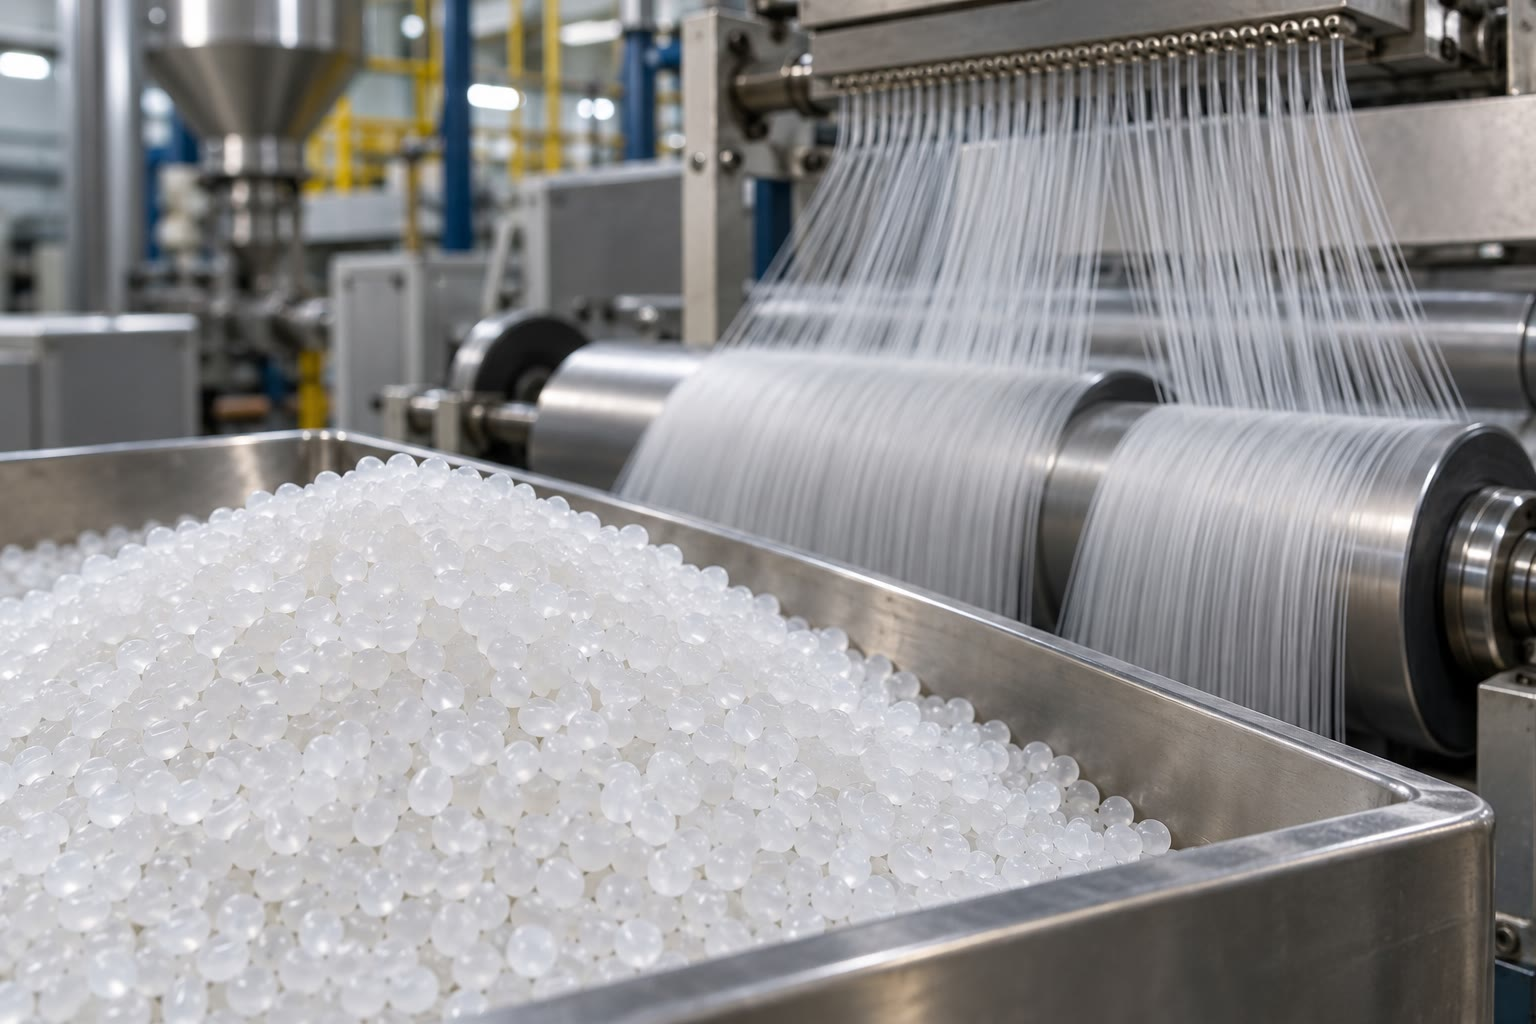
\includegraphics[width=0.58\linewidth]{images/book3/ai/b2-29-pellets.jpg}

{\small Butiran \omterm{def:b2:polymer-synthesis:polymer}{polimer} di sebuah pabrik, bentuk penjualan termoplastik, dan
serat yang ditarik dari nosel pemintal ke rol-rol yang berputar di belakangnya
(ilustrasi).}
\end{omfigure}

\begin{history}[Rendemen 99~\% tidaklah cukup]
\begin{minipage}[t]{0.2\linewidth}
\vspace{0pt}
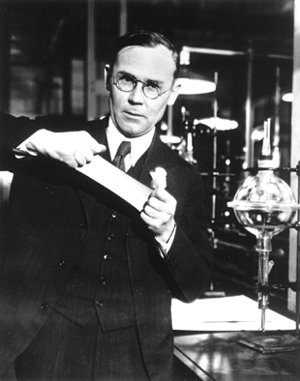
\includegraphics[width=\linewidth]{images/book3/carothers.jpg}
\end{minipage}\hfill
\begin{minipage}[t]{0.76\linewidth}
\vspace{0pt}
Wallace Carothers, seorang pengajar universitas muda yang direkrut ke sebuah
laboratorium industri untuk penelitian dasar, membangun molekul-molekul
panjang dari reaksi-reaksi yang sudah dikenal, dan hasil-hasilnya sangat
mendukung gagasan yang ketika itu masih diperdebatkan bahwa \omterm{def:b2:polymer-synthesis:polymer}{polimer} adalah
molekul biasa, hanya saja sangat panjang. Timnya membuat poliester, lalu,
sejak 1934, poliamida; persamaan yang menyandang namanya menjelaskan mengapa
hanya \omterm{def:b2:continuous-reactors:conversion}{konversi} yang ekstrem yang menghasilkan serat. Nilon mulai diproduksi
pada tahun 1939. (Foto: fotografer tidak diketahui, domain publik;
Wikimedia Commons.)
% ledger: hist:polyamides-1934, hist:nylon-production-1939
\end{minipage}
\end{history}

\begin{safety}{\ghs[5mm]{GHS01}\,\ghs[5mm]{GHS02}\,\ghs[5mm]{GHS05}\,\ghs[5mm]{GHS07}\,\ghs[5mm]{GHS08}\,\ghs[5mm]{GHS09}}
Stirena mudah terbakar dan membahayakan kesehatan. Dibenzoil peroksida
adalah pengoksidasi yang eksplosif jika kering dan disimpan dalam keadaan
lembap dan sejuk. Heksana-1,6-diamina dan asam heksanadioat korosif terhadap
mata.
% ledger: ghs:styrene, ghs:BPO, ghs:hexanediamine, ghs:adipic-acid
\end{safety}

\section{Latihan}

\begin{exercise}[$\star$]\label{exo:b2:polymer-synthesis:1}
Gambarlah \omterm{def:b2:polymer-synthesis:polymer}{satuan ulang} polietena, polipropena, poli(vinil klorida), polistirena, dan nilon-6,6.
\end{exercise}

\begin{exercise}[$\star$]\label{exo:b2:polymer-synthesis:2}
Pertumbuhan bertahap atau rantai: PET dari etana-1,2-diol dan asam
benzena-1,4-dikarboksilat; polistirena; nilon-6,6; poli(metil metakrilat);
poli(asam laktat) dari asam 2-hidroksipropanoat?
\end{exercise}

\begin{exercise}[$\star$]\label{exo:b2:polymer-synthesis:3}
Sebuah polistirena mempunyai $\bar X_n = 1000$. Hitunglah $\bar M_n$, dengan mengabaikan gugus-gugus ujung.
\end{exercise}

\begin{exercise}[$\star$]\label{exo:b2:polymer-synthesis:4}
Sebuah rantai polipropena yang digambar sebagai zig-zag planar mempunyai
gugus-gugus metil pada sisi pembaca, lalu menjauh, lalu mendekat, lalu
menjauh, dan seterusnya. Sebutkan \omterm{def:b2:polymer-synthesis:tacticity}{taktisitasnya}. Dapatkah rantai itu
mengkristal?
\end{exercise}

\begin{exercise}[$\star\star$]\label{exo:b2:polymer-synthesis:5}
Sebuah sampel adalah campuran dua fraksi bermassa sama, dengan massa molar
\qty{10}{kg/mol} dan
\qty{100}{kg/mol}. Hitunglah $\bar M_n$, $\bar M_w$, dan \omterm{def:b2:polymer-synthesis:averages}{dispersitasnya}.
\end{exercise}

\begin{exercise}[$\star\star$]\label{exo:b2:polymer-synthesis:6}
Hitunglah $\bar X_n$ untuk \omterm{def:b2:polymer-synthesis:step-chain}{polimerisasi pertumbuhan bertahap} yang berimbang pada $p = 0.98$ dan $p = 0.995$.
\end{exercise}

\begin{exercise}[$\star\star$]\label{exo:b2:polymer-synthesis:7}
Sebuah diasam dan sebuah diamina dicampur dengan kelebihan 1~\% (dalam mol)
diamina. Berapakah $\bar X_n$ terbesar yang dapat dicapai?
\end{exercise}

\begin{exercise}[$\star\star$]\label{exo:b2:polymer-synthesis:8}
Dalam sebuah polimerisasi radikal, konsentrasi inisiator dilipatduakan.
Dengan faktor berapakah laju polimerisasi dan \omterm{def:b2:polymer-synthesis:chain-length}{panjang rantai kinetik}
berubah?
\end{exercise}

\begin{exercise}[$\star\star$]\label{exo:b2:polymer-synthesis:9}
Poli(vinil klorida) bersifat kaku; selang taman yang terbuat darinya lentur
karena mengandung pemlastis, yaitu molekul kecil yang tercampur di antara
rantai-rantai. Jelaskan dengan transisi kaca.
\end{exercise}

\begin{exercise}[$\star\star\star$]\label{exo:b2:polymer-synthesis:10}
Tunjukkan bahwa sebaran massa Flory $w_x = x(1-p)^2p^{\,x-1}$, dipandang
sebagai fungsi $x$ yang kontinu, mencapai nilai terbesar pada $x = -1/\ln p$,
dan bahwa nilai ini dekat dengan $\bar X_n$ jika $p$ dekat dengan 1.
\end{exercise}

\begin{exercise}[$\star\star\star$]\label{exo:b2:polymer-synthesis:11}
PET dibuat dalam dua tahap: dimetil benzena-1,4-dikarboksilat dengan
etana-1,2-diol berlebih menghasilkan bis(2-hidroksietil)
benzena-1,4-dikarboksilat dan metanol; lalu diester ini dipanaskan dalam
vakum dan berpolimerisasi, sambil melepaskan etana-1,2-diol. Tuliskan kedua
tahap itu dan jelaskan bagaimana tahap kedua memecahkan masalah
stoikiometri persamaan Carothers.
\end{exercise}

\begin{exercise}[$\star\star\star$]\label{exo:b2:polymer-synthesis:12}
Dalam kopolimerisasi radikal \omterm{def:b2:polymer-synthesis:polymer}{monomer} 1 dan 2, komposisi sesaat \omterm{def:b2:polymer-synthesis:copolymer}{kopolimernya}
diberikan oleh $\dfrac{\mathrm d[\mathrm M_1]}{\mathrm d[\mathrm M_2]} = \dfrac{[\mathrm M_1](r_1[\mathrm M_1]
+ [\mathrm M_2])}{[\mathrm M_2]([\mathrm M_1] + r_2[\mathrm M_2])}$, dengan $r_1$ dan $r_2$
rasio kereaktifan (data latihan: $r_1 = 2.0$, $r_2 = 0.5$). Hitunglah rasio
satuan-satuan dalam \omterm{def:b2:polymer-synthesis:copolymer}{kopolimer} yang terbentuk dari umpan ekuimolar. Apa yang
terjadi jika $r_1 = r_2 = 0$?
\end{exercise}

\section{Soal: Nilon-6,6 per Kilogram}

\begin{problem}[{Soal akhir pekan --- monomer dan garam nilon, persamaan
Carothers, ketakseimbangan yang disengaja, sebaran Flory, dan air yang
dilepaskan}]
\label{pb:b2:polymer-synthesis:1}
Nilon-6,6 dibuat dari heksana-1,6-diamina dan asam heksanadioat. Gugus-gugus
ujung diabaikan di seluruh soal. Massa molar (\unit{g/mol}): C 12.011,
H 1.008, N 14.007, O 15.999.
% ledger: aw:C, aw:H, aw:N, aw:O, ghs:hexanediamine, ghs:adipic-acid

\medskip
\noindent\textbf{Bagian I --- \omterm{def:b2:polymer-synthesis:polymer}{Monomer} dan \omterm{def:b2:polymer-synthesis:polymer}{satuan ulang}.}
\begin{enumerate}
  \item Tuliskan rumus kedua \omterm{def:b2:polymer-synthesis:polymer}{monomer}.
  \item Tuliskan persamaan pembentukan satu ikatan amida.
  \item \omterm{def:b2:polymer-synthesis:polymer}{Monomer-monomer} itu mula-mula digabungkan sebagai garam 1\,:\,1,
        yang dikristalkan dari larutan. Mengapa?
  \item Tuliskan \omterm{def:b2:polymer-synthesis:polymer}{satuan ulang} nilon-6,6, rumusnya, dan massa molarnya.
  \item Berapakah massa molar rata-rata $M_0$ satuan turunan \omterm{def:b2:polymer-synthesis:polymer}{monomer} dalam rantai?
  \item Apa yang dihitung oleh kedua bilangan dalam nama ``6,6''?
\end{enumerate}

\medskip
\noindent\textbf{Bagian II --- Persamaan Carothers.}
\begin{enumerate}[resume]
  \item Hitunglah $\bar X_n$ dan $\bar M_n$ pada $p = 0.98$.
  \item Hal yang sama pada $p = 0.99$.
  \item Jelaskan ungkapan ``rendemen 99~\% tidaklah cukup''.
  \item Kemajuan reaksi berapakah yang menghasilkan $\bar M_n = \qty{10}{kg/mol}$?
  \item Bagaimana kemajuan reaksi didorong setinggi itu dalam praktik?
  \item Mengapa \omterm{def:b2:polymer-synthesis:polymer}{monomer-monomernya} harus sangat murni?
\end{enumerate}

\medskip
\noindent\textbf{Bagian III --- Ketakseimbangan yang disengaja.}
\begin{enumerate}[resume]
  \item Diamina dipakai dengan kelebihan molar 1~\%. Hitunglah $r$.
  \item Hitunglah $\bar X_n$ dan $\bar M_n$ terbesar yang kemudian dapat dicapai.
  \item Hitunglah $\bar X_n$ pada $p = 0.99$ dengan ketakseimbangan ini.
  \item Gugus manakah yang mengakhiri rantai-rantai di akhir reaksi?
  \item Sedikit asam etanoat kadang-kadang ditambahkan. Apa pengaruhnya pada rantai-rantai?
  \item Mengapa sebuah produsen sengaja membatasi panjang rantai?
\end{enumerate}

\medskip
\noindent\textbf{Bagian IV --- Sebaran dan neraca massa.}
\begin{enumerate}[resume]
  \item Untuk campuran berimbang pada $p = 0.99$, tentukan \omterm{def:b2:polymer-synthesis:averages}{dispersitasnya}.
  \item Hitunglah $\bar M_w$ pada $p = 0.99$.
  \item Pada $p = 0.99$, berapa fraksi molekul, dan berapa fraksi massa,
        yang masih berupa \omterm{def:b2:polymer-synthesis:polymer}{monomer} yang belum bereaksi?
  \item Di dekat panjang rantai berapakah sebaran massanya paling besar?
  \item Hitunglah massa air yang dilepaskan per kilogram nilon-6,6.
  \item Mengapa pemintalan leleh memerlukan $\bar M_n$ di dalam sebuah rentang tertentu?
  \item Nyatakan kemajuan reaksi yang menghasilkan $\bar M_n = \qty{20}{kg/mol}$
        untuk campuran berimbang.
\end{enumerate}
\end{problem}
